\documentclass[11pt]{article}
\usepackage[margin=1in]{geometry}
\usepackage[T1]{fontenc}
\usepackage{lmodern}
\usepackage{booktabs}
\usepackage{graphicx}
\usepackage{amsmath}
\usepackage{xcolor}
\usepackage{xurl}
\usepackage{hyperref}
\usepackage{enumitem}
\setlist{nosep}
\hypersetup{colorlinks=true,linkcolor=blue!50!black,urlcolor=blue!50!black}
\graphicspath{{reports/caa_pt_figures/}}
\newcommand{\astar}{\alpha^{*}}

\title{Preliminary Study, Part 2: Contrastive Activation Addition\\on the Pretrained Orpheus Hindi Model}
\author{cs-tts-steering project}
\date{November 5, 2026}

\begin{document}
\maketitle

\begin{abstract}
This extends the CAA pilot (\texttt{docs/reports/preliminary\_caa.pdf}) to the \emph{pretrained} Orpheus 3B Hindi model (\texttt{canopylabs/3b-hi-pretrain-research\_release}, ``PT''), which has no named voices. Positives are the 100 natural TV recordings of \texttt{Listening\_Examples\_100}; negatives are the model's own (on-policy) generations from the same Devanagari/English transcripts. The steering vector $v=\bar h_{\text{natural}}-\bar h_{\text{PT}}$ was built from 69 training pairs. Evaluation is a three-way comparison with one model: Natural vs.\ PT base vs.\ PT steered. As in the pilot, a linear natural-vs-PT direction exists at every site (held-out AUC median $1.0$, permutation 95th percentile $\le0.63$). The selected configuration (layer 27 attention output, mean-pooled $v$, $\astar=1$) moves an external natural-vs-PT classifier (M1) beyond a random vector of the same norm on the 19 test utterances ($+0.79$ log-odds, $p=.023$), but \textbf{not significantly beyond the unsteered baseline} ($+0.40$, 95\% CI $[-0.49,1.28]$). Similarity to the paired natural clip (M2) and prosody distance (M3) move in the right direction but are not significant. In-sample on all 100 utterances, M1 improves clearly ($+0.84$, $p=5\times10^{-5}$) and M2/M3 trend better ($p\approx.08$), while voice quality worsens (HNR $-1.1$\,dB, jitter and shimmer up) and NISQA is unchanged. The pre-registered failure guardrail admitted no configuration; we recalibrated it to the measured sampling variance of the unsteered model. On test the steered model still fails the failure-rate and WER guardrails, the latter because of one clip. The objective verdict is \textbf{no-go}, with a weak positive signal. In an informal team listening session, the steered clips sounded somewhat more natural, but in several clips the spoken words were wrong or fragmented. A clip-level analysis suggests this comes mostly from the transcripts and from the unsteered model itself, not from steering (\S\ref{sec:listening-feedback}). Filtering the training pairs, or tracing errors back to the transcripts, is the next step.
\end{abstract}

\section{Question and design changes from the pilot}
The pilot steered fine-tuned models with a fixed voice and used their default outputs as negatives. Here we ask whether the same mechanism improves the \emph{pretrained} Orpheus checkpoint, whose baseline output is the model's own unprompted delivery. The changes from the pilot are:
\begin{itemize}
\item \textbf{Model:} Orpheus Hindi PT, revision b813fee6, bf16. Text-only prompt (no voice prefix), so the speaker varies per clip.
\item \textbf{Negatives:} on-policy PT generations, one sample per transcript at seed 1234 (decoding $t=0.6$, top-$p$ 0.9, repetition penalty 1.1, batch size 1). These same clips are the ``PT base'' condition.
\item \textbf{Input:} Devanagari/English transcripts only.
\item \textbf{Split:} the pilot's split, reused as is (76 train including 16 dev, 19 test, 5 excluded; seed 20261029).
\item \textbf{Evaluation:} one model, three groups (Natural, PT base, PT steered), plus a random-vector control on test. Metrics are the partner summary's figure set (\texttt{preliminary\_summary.pdf}), NISQA-TTS, and the pilot's M1--M3.
\end{itemize}
The listening package is a new folder with the same per-utterance layout as \path{Listening_Examples_100} (\S\ref{sec:listening}).

\section{Method}
\subsection{Teacher forcing and the PT prefix}
In all 100 base generations, the PT model emitted the same start-of-audio prefix as the fine-tuned model, \texttt{[128261, 128257]}, and no non-audio tokens inside or after the audio. Teacher forcing therefore uses \texttt{128259} + tok(text) + \texttt{128009, 128260, 128261, 128257} + SNAC audio tokens + \texttt{128258}. Natural clips were mixed to mono, resampled to 24\,kHz and SNAC-encoded; PT clips were re-encoded from their wavs, so both classes go through the same encoder. A SNAC round trip on 9 real clips was exact.

\subsection{Base generations and contrast set}
Of the 100 base generations, 10 ran to the token budget without ending speech (7 train, 1 test, 2 of the excluded utterances). Several are short inputs at the 8\,s minimum budget, so they are runaways, not truncation. The 7 failed train negatives were dropped together with their natural clip, leaving \textbf{69 train pairs} for $v$.

\subsection{Diagnostics, selection and test}
Sites, pooling, norm-preserving injection ($\tilde h=h+\alpha v$, rescaled to $\|h\|$) and statistics are the pilot's. Following option (a) of the plan, we ran the lean diagnostics (probes, held-out projection AUC against a permutation control, audio-token NLL) and then a dev sweep restricted to attention \texttt{o\_proj}, mean-pooled sites, the only family usable in the pilot:
\begin{itemize}
\item Sweep 1: the 6 shortlisted layers, each at $\alpha\in\{0.5,1,2\}$, on the 16 dev utterances.
\item Sweep 2: the top-2 and top-3 layers combined, at the same $\alpha$ values.
\end{itemize}
The selection rule and composite score are the pilot's. A clip counts as a failure if it has no end-of-speech token, hits the budget, or lasts less than half or more than twice its seed-1234 base clip. The selected vector was then applied to all 100 utterances, and a random vector of the same norm at the same site and $\alpha$ to the 19 test utterances.

\subsection{Metrics}
\begin{itemize}
\item \textbf{Summary figure metrics}, computed with the partner's code: Whisper-large-v3 WER/CER and ASR speaking rate, Praat prosody and voice quality, syllable-nucleus rate, WavLM-SV within-group speaker consistency.
\item \textbf{NISQA-TTS:} official repository at commit fe84f0f2, run in a separate environment. The checkpoint pickle was inspected before loading and also loads with \texttt{weights\_only=True}.
\item \textbf{M1:} log-odds of a logistic natural-vs-PT classifier on WavLM-base-plus embeddings, trained on the train utterances (held-out AUC 1.000).
\item \textbf{M2:} WavLM cosine similarity to the paired natural clip.
\item \textbf{M3:} IQR-scaled prosody distance to the paired natural clip (lower is better).
\item \textbf{Guardrails:} WER/CER, S-SIM to the base clip, failure rate.
\end{itemize}
The 19 test utterances are the primary result. All-100 numbers are reported as \emph{in-sample}, because $v$ and the M1 classifier used the train utterances.

\section{Results}
\subsection{Diagnostics}
\begin{center}
\begin{tabular}{lcc}
\toprule
 & Orpheus PT & Pilot Orpheus FT \\
\midrule
Sites with probe accuracy $=1.0$ & 78/112 & 82/112 \\
Probe accuracy, permuted labels & 0.475 & 0.49 \\
Held-out projection AUC, min / median & 0.743 / 1.0 & 0.89 / -- \\
Permutation AUC, mean / max 95th pct. & 0.494 / 0.625 & 0.49 / 0.62 \\
Cohen's $d$, median (resid.\ / attn.) & 4.4 / 4.5 & 5.7 / 5.8 \\
$\|v\|/\|h\|$, median (resid.\ / attn.) & 0.31 / 0.67 & 0.28 / 0.73 \\
Audio-token NLL, natural vs.\ synthetic (nats) & 5.69 vs.\ 2.69 & 5.93 vs.\ 3.17 \\
\bottomrule
\end{tabular}
\end{center}
The direction is far above chance at every site. As in the pilot, separation is close to trivial: natural audio is about twice as surprising to the model, and speaker and channel differ. Diagnostics alone therefore cannot choose a site. The shortlist (all AUC 1.0) was layers 24, 20, 27, 23, 22 and 26.

\subsection{Selection}
\textbf{Under the pre-registered rule, no configuration was admissible} (0 of 27). The dev base failed on 0 of 16 clips, so the failure threshold was 5\%, and every steered configuration failed on at least 12.5\%. To test whether this reflects steering or sampling, we resampled the \emph{unsteered} model at seeds 1235 and 1236 on the same 16 utterances. By the same definition it failed on \textbf{7/32 = 21.9\%} (3 runaways, 4 duration ratios), on the same utterances that fail under steering. Because PT draws a new speaker for every sample, the duration-ratio test against a single base clip mostly measures sampling variance. We therefore recalibrated the threshold to $\max(5\%,\ \text{base},\ 21.9\%)$. This is a post-hoc deviation; the strict outcome is reported alongside it.

\begin{center}
\resizebox{\textwidth}{!}{%
\begin{tabular}{lcccccccc}
\toprule
Config (dev) & Fail & WER & CER & S-SIM & $\Delta$M1 & $\Delta$M2 & $\Delta$M3 & Admissible \\
\midrule
L20, $\alpha=0.5$ & .188 & .741 & .606 & .838 & +0.88 & $-$.005 & $-$.121 & yes \\
\textbf{L27, $\alpha=1$} & \textbf{.125} & \textbf{.767} & \textbf{.614} & \textbf{.876} & \textbf{+0.95} & \textbf{+.027} & \textbf{$-$.163} & \textbf{yes, selected} \\
L27, $\alpha=2$ & .250 & .800 & .629 & .895 & +1.47 & +.014 & $-$.053 & no (fail) \\
L27+L20, $\alpha=0.5$ & .125 & .704 & .519 & .882 & +0.61 & +.006 & $-$.190 & yes \\
L27+L20+L24, $\alpha=0.5$ & .188 & .794 & .604 & .908 & +1.09 & +.022 & +.030 & yes \\
L26, $\alpha=0.5$ & .188 & .878 & .680 & $\approx$.86 & +1.27 & $\approx$+.02 & $-$.15 & no (WER) \\
\midrule
Dev PT base & 0 & .814 & .602 & -- & -- & -- & -- & \\
\bottomrule
\end{tabular}}
\end{center}
Four configurations passed the recalibrated rule, and \textbf{layer 27 attention output at $\astar=1$} had the best composite score (0.527). Stronger or multi-layer steering raised either failures or WER. Across sweep-1 sites, steering effect and diagnostic separation were not positively related (correlation $-0.26$). The full table is in the run's \texttt{report.md}.

\subsection{Test set (19 utterances)}
\begin{center}
\resizebox{\textwidth}{!}{%
\begin{tabular}{lcccc}
\toprule
Metric (median unless noted) & Natural & PT base & PT steered & Random control \\
\midrule
Failures (of 19) & 0 & 1 & 5 & 3 \\
WER corpus & .945 & .718 & 1.235 (.717 w/o outlier) & .725 \\
CER corpus & .877 & .602 & .843 (.573 w/o outlier) & .614 \\
Syllable-nucleus rate (/s) & 4.20 & 3.20 & 3.23 & 3.60 \\
Duration (s) & 5.49 & 6.40 & 6.57 & 5.46 \\
Median F0 (Hz) & 220 & 129 & 149 & 137 \\
F0 range (st) & 19.9 & 6.3 & 9.3 & 7.3 \\
Internal pause (\%) & 17.6 & 18.8 & 21.3 & 19.7 \\
HNR (dB) & 8.7 & 15.5 & 15.0 & 14.7 \\
NISQA-TTS & 2.94 & 3.62 & 3.57 & 3.58 \\
Speaker consistency (mean pair cosine) & .732 & .834 & .848 & .838 \\
M1 logit (mean) & 5.38 & $-$4.25 & $-$3.85 & $-$4.64 \\
M2 (mean) & -- & .676 & .696 & .661 \\
M3 (mean, lower better) & -- & 1.015 & .951 & 1.097 \\
S-SIM to PT base (mean) & -- & -- & .883 & .889 \\
\bottomrule
\end{tabular}}
\end{center}

\noindent Paired differences, mean [95\% bootstrap CI], Wilcoxon $p$, $n=19$:
\begin{center}
\resizebox{\textwidth}{!}{%
\begin{tabular}{lccc}
\toprule
 & Steered $-$ base & Random $-$ base & Steered $-$ random \\
\midrule
M1 & +0.40 [$-$0.49, 1.28], $p=.44$ & $-$0.39 [$-$1.01, 0.24], $p=.42$ & \textbf{+0.79 [0.18, 1.34], $p=.023$} \\
M2 & +0.020 [$-$0.038, 0.084], $p=.83$ & $-$0.014, $p=.54$ & +0.034, $p=.33$ \\
M3 & $-$0.064 [$-$0.28, 0.12], $p=.89$ & +0.082, $p=.52$ & $-$0.147, $p=.20$ \\
NISQA & $-$0.06 [$-$0.34, 0.25], $p=.74$ & $-$0.15, $p=.54$ & +0.09, $p=.74$ \\
Median F0 (Hz) & +9.0 [$-$8.3, 23.8], $p=.12$ & $-$2.5, $p=.47$ & +11.5, $p=.11$ \\
Failure & +0.21 [0.05, 0.42] & +0.11 [0, 0.26] & +0.11 \\
\bottomrule
\end{tabular}}
\end{center}
The only steered-minus-base interval that excludes zero is the failure rate. Steering beats a random vector on M1, so the effect is specific to $v$, but it is too small to separate from the baseline on 19 utterances. Guardrails on test: S-SIM passes. WER and CER fail because of a single clip, \texttt{train\_1693\_0}: the steered clip ends properly but runs 16.0\,s against 5.9\,s for base (clip WER 8.1). Without it, steered WER/CER are .717/.573 against .726/.606 for base. The failure rate fails, at 26\% against the 21.9\% threshold. Only 1 of the 5 steered failures is a runaway; the other 4 are duration-ratio flags. One of them, \texttt{train\_1753\_4}, is a properly ended 1.6\,s steered clip whose \emph{base} was the runaway.

\begin{figure}[ht]
\centering
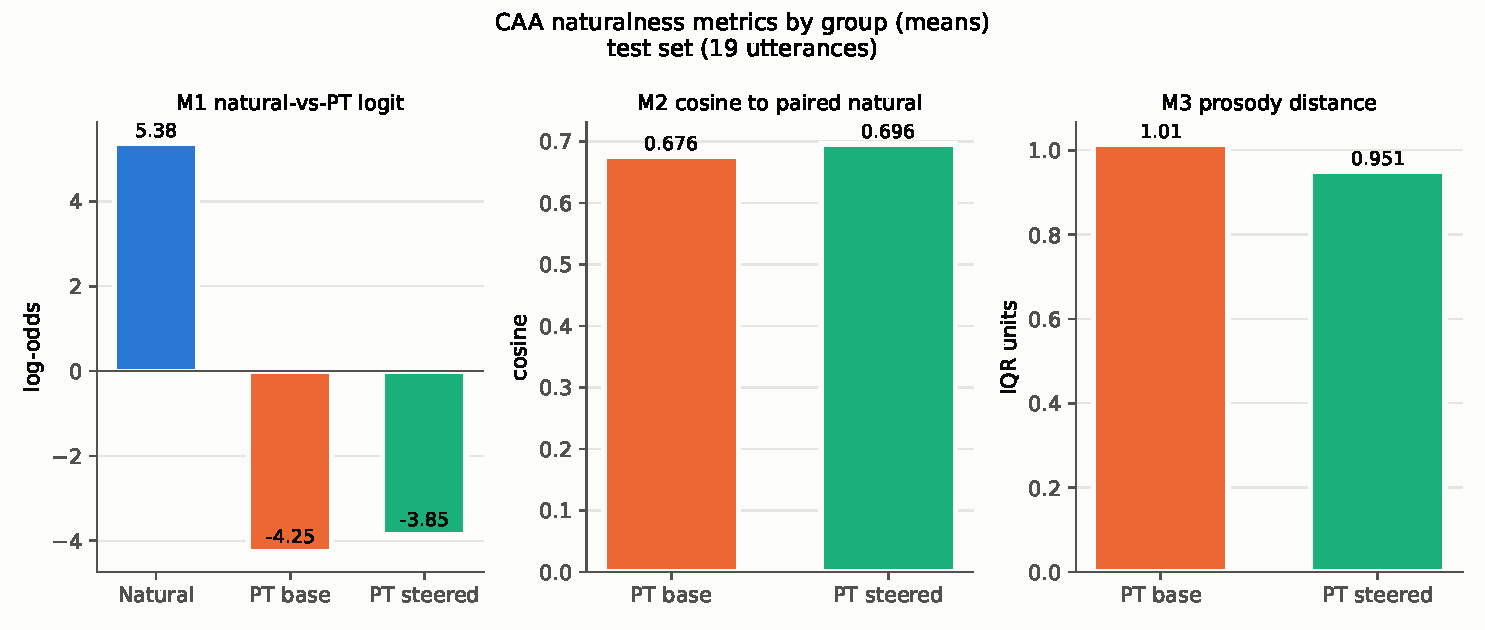
\includegraphics[width=\textwidth]{08_naturalness_m1_m3_test19.pdf}
\caption{M1--M3 on the test set. M2 and M3 compare each generated clip with its paired natural clip, so Natural has no bar.}
\end{figure}
\begin{figure}[ht]
\centering
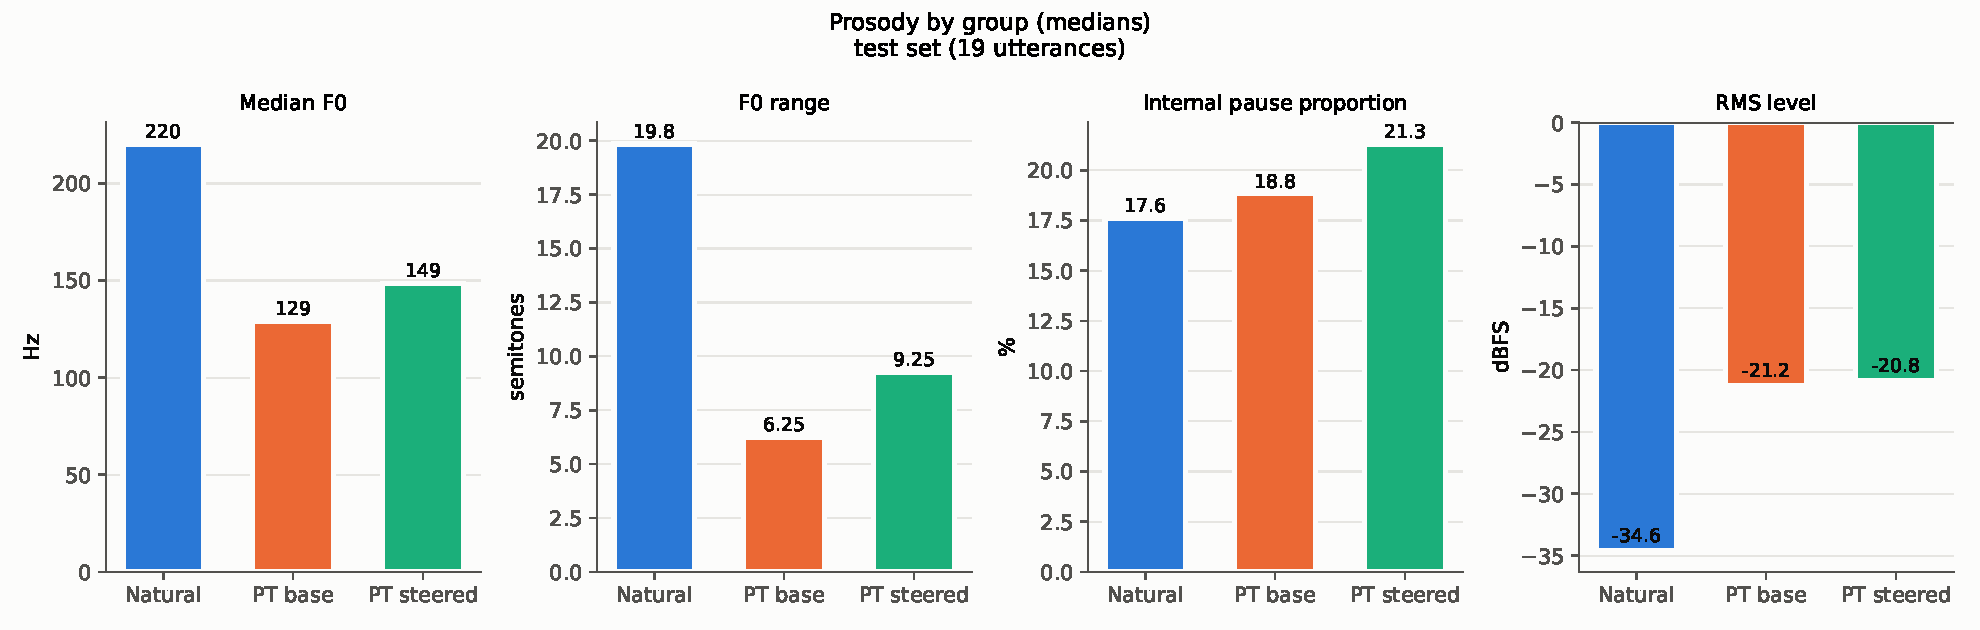
\includegraphics[width=\textwidth]{04_prosody_test19.pdf}
\caption{Prosody on the test set (medians).}
\end{figure}

\subsection{All 100 utterances (in-sample)}
\begin{center}
\resizebox{\textwidth}{!}{\begin{tabular}{lccc}
\toprule
Metric & Natural & PT base & PT steered \\
\midrule
Failures / runaways only & 0 / 0 & 10 / 10 & 18 / 3 \\
WER median / corpus & .750 / .880 & .750 / .817 & .756 / .988 \\
Syllable-nucleus rate (/s) & 4.02 & 3.23 & 3.68 \\
Median F0 (Hz) / F0 range (st) & 225 / 19.8 & 141 / 7.4 & 142 / 8.2 \\
Internal pause (\%) & 18.3 & 19.6 & 14.8 \\
Jitter / shimmer / HNR (dB) & .024 / .127 / 8.6 & .019 / .081 / 14.8 & .020 / .088 / 13.5 \\
NISQA-TTS & 3.15 & 3.69 & 3.72 \\
Speaker consistency & .776 & .853 & .855 \\
M1 / M2 / M3 (means) & 5.69 / -- / -- & $-$4.87 / .655 / 1.049 & $-$4.03 / .680 / .983 \\
\bottomrule
\end{tabular}}
\end{center}
Steered $-$ base, $n=100$: M1 $+0.84$ [0.50, 1.21], $p=5\times10^{-5}$; M2 $+0.025$ [$-0.000$, 0.052], $p=.085$; M3 $-0.066$ [$-0.139$, 0.008], $p=.072$; syllable-nucleus rate $+0.43$/s, $p=.003$; HNR $-1.08$\,dB, $p=5\times10^{-4}$; jitter and shimmer up, $p<.02$; NISQA $+0.11$, $p=.10$. Runaways drop from 10 to 3, but duration-ratio flags rise, so total failures go from 10 to 18. These numbers are biased upward by in-sample use but are consistent in sign with the test set.

\subsection{Go/no-go}
\begin{center}
\begin{tabular}{lcc}
\toprule
Criterion & Test (19) & Verdict \\
\midrule
Direction exists (AUC vs.\ permutation) & 1.0 vs.\ 0.63 & pass \\
M1 specific to $v$ (vs.\ random) & +0.79, $p=.023$ & pass \\
M1 better than base & +0.40, CI includes 0 & fail \\
M2 / M3 better than base & n.s. & fail \\
S-SIM guardrail & .883 & pass \\
WER/CER guardrail & fails (one clip) & fail \\
Failure guardrail (recal.) & 26\% vs.\ 21.9\% & fail \\
\midrule
\textbf{Overall} & & \textbf{no-go (weak positive signal)} \\
\bottomrule
\end{tabular}
\end{center}

\subsection{Team listening feedback and content errors}\label{sec:listening-feedback}
An informal listening session by the team (Hindi--English bilinguals, not blind) gave two observations:
\begin{itemize}
\item The steered clips sound \emph{a bit more natural} than PT base. This agrees with the direction of M1--M3.
\item In several clips the \emph{content is wrong or fragmented}: words are missing, garbled or not the words of the transcript.
\end{itemize}
To see where the content errors come from, we compared clip-level CER (Whisper-large-v3 against the input transcript) for the three groups, over all 100 utterances. CER is only a rough proxy for what listeners hear, especially for Hinglish.
\begin{itemize}
\item \textbf{PT base already has poor content.} Its corpus CER on test is 0.60, so many unsteered clips already contain wrong or missing words.
\item \textbf{Steering does not make content worse overall.} Steering raised CER by more than 0.1 in 19\% of utterances and lowered it by more than 0.1 in 28\%. The size of the change is unrelated to transcript quality (Spearman $\rho=0.0$ with natural-clip CER). The exception is \texttt{train\_1693\_0}, whose steered clip runs 2.7 times as long as base and whose CER rises from 0.55 to 4.4; that error is caused by steering.
\item \textbf{The transcripts often do not match the natural recordings.} Whisper on the \emph{natural} clips disagrees strongly with our transcripts: median CER 0.61, with 38 of 76 train utterances above 0.6 and 17 above 0.8. For \texttt{train\_1574\_0} the CER is 14.5, so the transcript and recording barely correspond. Some of this is Whisper's weakness on Hinglish, but not all of it.
\item \textbf{Bad transcripts and poor model content go together.} Utterances where Whisper disagrees with the transcript on the natural clip are also the ones where PT's own output scores worst (Spearman $\rho=0.58$ for base, $0.56$ for steered). Mismatched or malformed text input gives poor output whether or not we steer.
\end{itemize}
This also matters for the vector itself. When a natural clip does not match its transcript, the teacher-forced natural activations encode ``audio that does not fit the text''. $v$ then partly points toward text--audio mismatch, which would push generations away from the transcript. This agrees with the high natural NLL (5.69 vs.\ 2.69 nats) and with the pilot's NLL confound. The upshot is that the training pairs should be filtered, or the transcripts fixed, before the next run (\S\ref{sec:next}).

\section{Discussion}
\paragraph{Same picture as the pilot, with one difference.} The direction exists, is causal, and is specific to $v$. But on the test set it does not bring output measurably closer to the paired natural recording. Unlike the pilot, M2 and M3 here move in the right direction in-sample, with $p\approx.08$, so the PT model may be somewhat more steerable toward natural delivery than the fine-tuned models.
\paragraph{What the vector changes.} Steering raises F0 level and range and the syllable rate, moving toward the natural pool. It also lowers HNR and raises jitter and shimmer. Natural TV audio has lower HNR and higher jitter than TTS, so these changes may partly be steering toward the TV channel rather than toward delivery. NISQA, a learned quality score, is flat: it neither rewards nor penalises the change.
\paragraph{Sampling variance dominates the guardrails.} PT draws a new speaker for each sample, and even unsteered resamples fail the duration-ratio test 22\% of the time. Single-seed comparisons against one base clip are therefore noisy. A fair test needs several seeds per utterance and failure criteria that do not depend on one reference clip.
\paragraph{WER is a weak proxy.} Natural speech has a higher WER than PT (corpus .945 vs.\ .718), as in the partner summary, so higher WER does not necessarily mean less intelligible speech.
\paragraph{Transcripts.} The caveat from the pilot applies: the Devanagari/English inputs went through lossy romanization and transliteration, so they do not fully match what was said in the natural clips. Here the mismatch is measurable (natural-clip CER median 0.61) and is the likeliest source of the wrong or fragmented content listeners heard (\S\ref{sec:listening-feedback}).

\section{Limitations}
\begin{itemize}
\item 19 test utterances, one seed per utterance and condition, and a random speaker per clip. Small effects cannot be resolved.
\item The failure guardrail was recalibrated after sweep 1. Under the strict rule, nothing would have been selected.
\item Several metric deviations from the partner summary: natural audio resampled with torchaudio rather than \texttt{resample\_poly}; NISQA run with newer library versions than its pins, with clips under 0.3\,s left unscored (1 clip); small stand-ins for two scipy functions used only by unreported features.
\item The mechanistic projection check from the pilot was not run.
\item Human listening so far is informal and not blind. Naturalness is judged only by bilingual listeners (\texttt{AGENTS.md}); a blind test is still needed.
\item Content errors were assessed with Whisper CER, which is unreliable for Hinglish and cannot separate transcript errors from ASR errors.
\end{itemize}

\section{Next steps}\label{sec:next}
\begin{enumerate}
\item \textbf{Find mismatched transcripts.} Rank the 100 utterances by Whisper CER on the natural clip and have a Hindi speaker check the worst 20 or so, separating transcript errors from ASR errors.
\item \textbf{Rebuild $v$ from clean pairs.} Drop flagged train pairs, rebuild the vector, and rerun only the final stage at the same site and $\alpha$ (about one GPU-hour). Compare content and naturalness with this run.
\item \textbf{Fix the transcripts at the source.} Correct flagged transcripts, or re-transcribe the natural audio directly into Devanagari/English instead of going through romanized text.
\item Blind A/B listening on \path{Listening_Examples_100_PT}, test utterances first. Include \texttt{train\_1693\_0}, and note per clip whether the words are wrong in base, steered or both.
\item Re-run base and steered with 3--5 seeds per utterance to separate steering from sampling variance, and define failure relative to the base distribution rather than one clip.
\item Reduce the channel confound, for example by building $v$ from natural clips matched to PT on loudness and band-limiting, or by subtracting a speaker/channel direction.
\end{enumerate}

\section{Listening package}\label{sec:listening}
On kedi at \path{/local/speech/users/sp4050/Listening_Examples_100_PT/}. It has the same 100 folder names as \texttt{Listening\_Examples\_100}. Each folder holds a copy of the natural clip, \texttt{TRANSCRIPT.txt}, \texttt{02\_OrpheusPT\_base.wav} and \texttt{03\_OrpheusPT\_steered.wav}, and is tagged with its split (19 test, 60 train, 16 dev, 5 excluded). The top level has \texttt{manifest.csv} (with SHA-256 per file), \texttt{utterances\_100.csv}, \texttt{READ\_ME.txt} and \texttt{listen.html} (three players per utterance).

\appendix
\section{Provenance}
\begin{itemize}
\item Run: \path{/local/speech/users/sp4050/outputs/caa_pt/20261105-1232_listening100/} (\texttt{report.md}, \texttt{report\_phase1.md}, \texttt{config.yaml}, \texttt{generations.jsonl}, \texttt{tables/}, \texttt{selection/}, \texttt{figures/}, \texttt{provenance/}).
\item Code: base commit a5240e0 plus the CAA-PT changes (\path{configs/caa_pt/pt.yaml}, \path{scripts/caa_pt_report.py}, and the config-driven pilot scripts). 11 unit tests pass.
\item Model revisions: Orpheus PT b813fee6, SNAC d73ad176. NISQA fe84f0f2, \texttt{nisqa\_tts.tar} sha256 c556a954\ldots.
\item Key numbers in this report were recomputed from \texttt{metrics/clips\_pt.csv} and match the run's \texttt{stats.json}.
\end{itemize}
\end{document}
